\section{An Introduction from the Dean} \shorttitle{The Jacobs Center for Lifelong Learning and Institutional Development}

Western industrialized nations have been undergoing fundamental changes in economic, cultural and social life. These changes are precipitated by more and more people reaching old and very old age, by markedly reduced birth rates, by living in an era of rapid knowledge turnover and by ever increasing globalization. Consequently, patterns of working, learning, and living need to change apace. This implies challenges for social institutions, including institutions of higher education, for corporations as well as for the individual. It is the goal of the Jacobs Center of Lifelong Learning and Institutional Development (JCLL) to do \textit{research} that contributes to the knowledge necessary to optimize the current transformations, and to provide \textit{education} and \textit{consulting} that support these transformations. Against the background of this historic constellation, the JCLL pursues the general aim to better understand individual and institutional conditions of \textit{productive adult development} and it does so from a systemic perspective (see below). Productive is defined in a broad sense that goes beyond the narrow economic understanding of productivity as exclusively linked to the contribution to the gross national product (cf. Staudinger, 1996).

%Over the past years, ``lifelong learning'' has become a rather overworked catchphrase, and sometimes even an empty shell. However, with regard to the current changes in Western industrialized societies, it has become more and more important for the individual and corporations alike to be able to continuously adapt to changing circumstances and environments. At the JCLL we have therefore opted for a definition of lifelong learning as one of three central developmental mechanisms, the other two being maturation/senescence and action. Learning in this sense encompasses formal as well as informal and incidental learning episodes. It addresses the knowledge and skills that are needed in personal, civic, social and professional life. Investigating lifelong learning at the JCLL is therefore part and parcel of the study of lifespan development. 


%The notion of lifelong learning within JCLL thus rests on Wilhelm von Humboldt's idea of education that is neither restricted to the learning of facts nor to learning in school. Humboldt proposed a notion of education that concerns the whole life course and all spheres of life. His notion of education also includes education in the sense of working on personality growth and maturation as well as the establishment of a value system that aims to not only further one's own good but also the common goal. This notion of ``Bildung'' (which is not properly captured by the English term education) and lifelong learning is very closely linked to the idea of optimizing human development in the sense of positive lives.
%\enlargethispage*{0.2cm}

%The JCLL \looseness=-1 focuses in its research on the analysis of \textit{development in context} and more specifically in the work context. By investigating human and organizational development in the work context, we aim to understand how individual (body and mind) and institutional conditions interact to produce outcomes on the individual as well as the organizational level. Interactionism forms the basis of our systemic model of adult development in the work context (see Figure \ref{fig:deanIntro}). Located in its center is the developing (aging) individual. In our model, we acknowledge that the individual as smallest system unit already comprises two dimensions: a mechanic and a pragmatic dimension (cf. Staudinger \& Pasupathi, 2000). 


%\begin{figure}[h]
 % \begin{center}
  %  \resizebox{0.5\textwidth}{!}{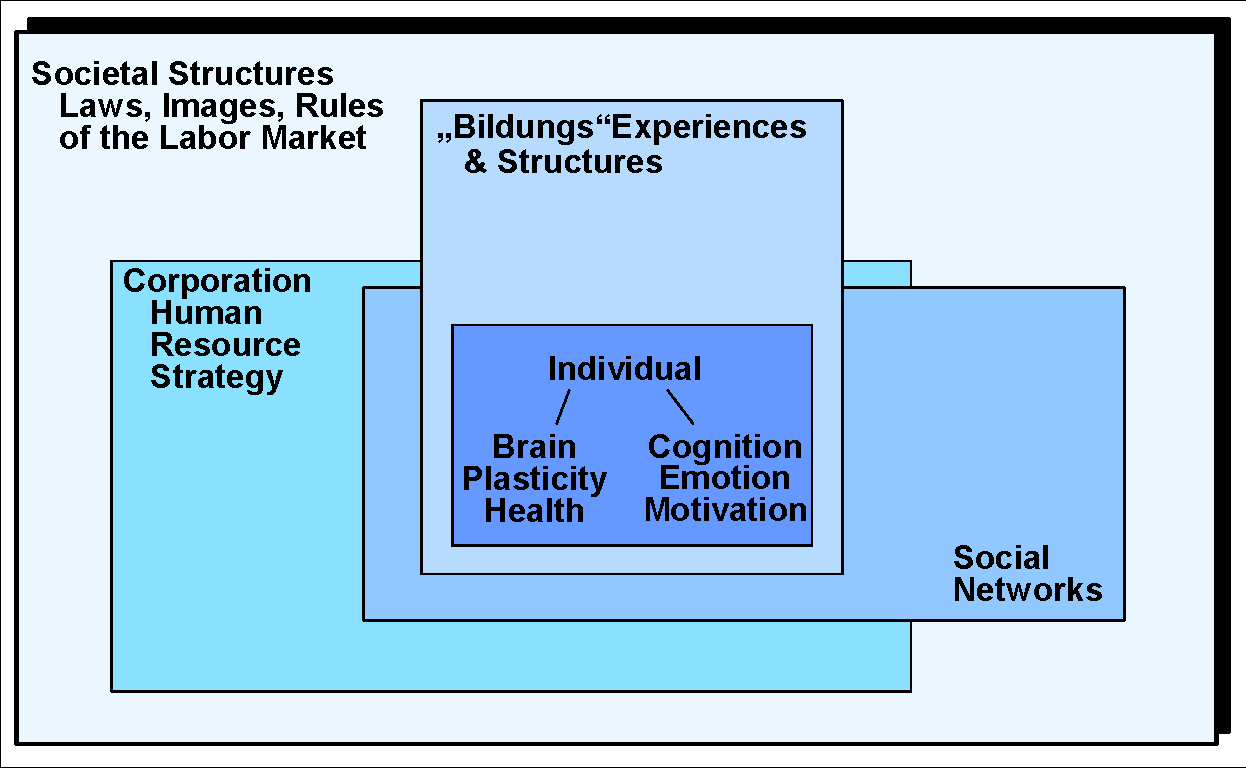
\includegraphics{deanUrsulaStaudingerIntro}}
   % \caption{Productive adult development at the Jacobs Center: A systemic approach (based on Staudinger, 2006).}
   % \label{fig:deanIntro}
  %\end{center}
%\end{figure}


\newpage
%The mechanic dimension refers to the fact that we all are biological beings with regard to our intelligence or cognition, our personality (motivation, emotion) and our social relations. This biological facet of our existence needs to be taken into account as facilitative and debilitating constraint to any intervention. At the same time, we are cultural and agentic beings, that is, there is a pragmatic dimension to human existence. Societal structures constrain and enable human development as well as individual choices and interpretations. 

%\begin{figure}[ht]
%  \begin{center}
%    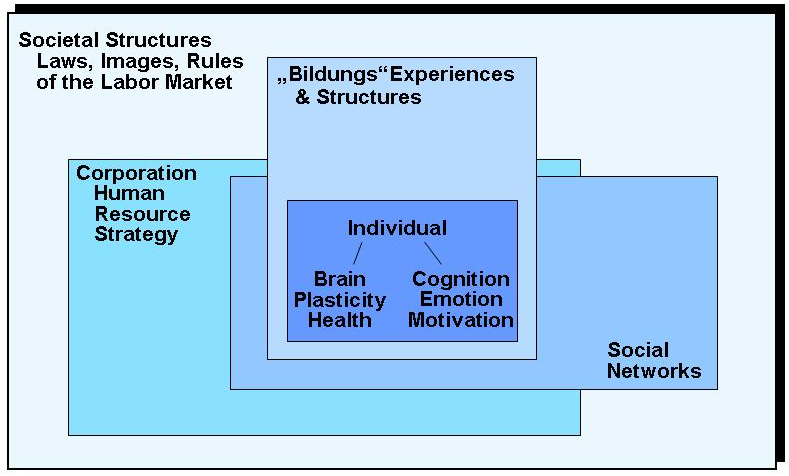
\includegraphics[width=7cm]{deanUrsulaStaudingerIntro.png}
%    \caption{Productive Adult Development at the Jacobs Center: A systemic approach (based on Staudinger, 2006).}\label{fig:deanIntro}
%   \end{center}
%\end{figure}



The developing individual is embedded in different important systems of influence that need to be kept in mind if the process of development is supposed to be productive. These systems are ``Bildungs'' experiences, social networks, the respective corporation with its approach to human resource development and finally the societal framework conditions such as the legal framework of work and education but also the images of aging and ``Bildung'' available in the public. In all these systems, changes have become necessary to accommodate the current transformative processes and enable successful lifelong learning and lifespan development. 


This systemic framework asks for multiple disciplines to be represented at the JCLL, such as Neuroscience and Human Performance, Lifespan Psychology, Health and Personality Psychology, Organizational Behavior (with a focus on learning in the work setting), Media and Communication Sciences (with a focus on images of aging, age-graded medial preferences and media competence), Business Administration, and Lifecourse Sociology and Economics.


The mutual \looseness=-1 dependencies of individual and social change are the focus of JCLL's joint research endeavors. For instance, the contribution of the Jacobs Center to the proposal of a Graduate School of the Social Sciences (BIGSSS) in the context of the Initiative for Excellence of the German Government (DFG / Wissenschaftsrat) lies exactly at the investigation of life-course and lifespan dynamics and their effect on individual and institutional or societal outcomes. Similarly, the interaction between the individual and the organization plays a central role in the first JCLL joint research proposal successful with the BMBF (Federal Ministry for Bildung and Research). In this project - that brings together all JCLL faculty under one common theme - we are interested in the matches and mismatches among employees' attitudes and competencies, the management strategies and work organization of the company as well the organizational climate with regard to the following domains: health promotion, training, images of aging, experience transfer, and adaptive competence. The central assumption is that individual as well as organizational outcomes (e.g., health, productivity) are best understood when taking into consideration the matches and mismatches between all possible combinations (Strategy - Climate, Climate - Employee, Employee - Strategy). Both a linear as well as a typological approach are considered as useful analytical tools. Five companies have agreed to participate. We will pursue a two-step sampling procedure: first we sample work units per company and second we sample individuals within each work unit. In order to keep the assessment protocol to a realistic length not all research domains will be assessed at each company. Rather, always two companies will have one domain in common. Thus, replication of findings across companies becomes possible. The research project, which will start in April 2007, is part of a program initiative by the BMBF revolving around innovative approaches to work security and health protection in the workplace. One of the results of this project will be a diagnostic toolbox for the identification of matches or mismatches in the domains of aging, learning, health, communication and adaptive capacity as well as application rules to be given to companies that want to work with the tool. 


Ursula M. Staudinger\\ 
Bremen, December 2006
